% Verifier-Anchored RL: design overview + prior-art survey + first results.
% A self-contained working-group deck (not the conference talk).
% Build: latexmk -pdf 2026-07-02-design-overview.tex
\documentclass[aspectratio=169]{beamer}

\usetheme{metropolis}
\metroset{block=fill}

\usepackage{amsmath,amssymb}
\usepackage{booktabs}
\usepackage{tikz}
\usetikzlibrary{arrows.meta,positioning,fit,backgrounds,shapes.misc}

\newcommand{\pitheta}{\pi_\theta}
\newcommand{\Qpsi}{Q_\psi}
\newcommand{\verbword}[1]{\texttt{#1}}

\title{Verifier-Anchored RL over a Frozen LLM}
\subtitle{Design, prior art, and first live results}
\date{July 2026}
\author{Alexander Towell}

\begin{document}

\maketitle

% ---------------------------------------------------------------- overview
\begin{frame}{What this is (and is not)}
  \begin{block}{The system}
    A \alert{tiny external controller} (verb head + pointer head + $Q$ head,
    a few million parameters) learns to orchestrate a \alert{frozen} LLM by
    issuing typed $(\text{verb}, \text{target})$ actions over a structured,
    nested reasoning forest. A \alert{symbolic verifier} is the only reward
    source.
  \end{block}
  \begin{itemize}
    \item \textbf{Not} o1 / DeepSeek-R1: RL never touches the LLM's weights
    \item \textbf{Not} a learned reward model: no PRM, ORM, critic, or
          LLM-judge anywhere in the reward path
    \item Training spine: off-policy value-based $Q$-learning; MCTS is a
          strictly additive accelerator and the test-time compute knob
  \end{itemize}
\end{frame}

% ---------------------------------------------------------------- architecture
\begin{frame}{Architecture: one action selects the operation and scopes the context}
  \centering
  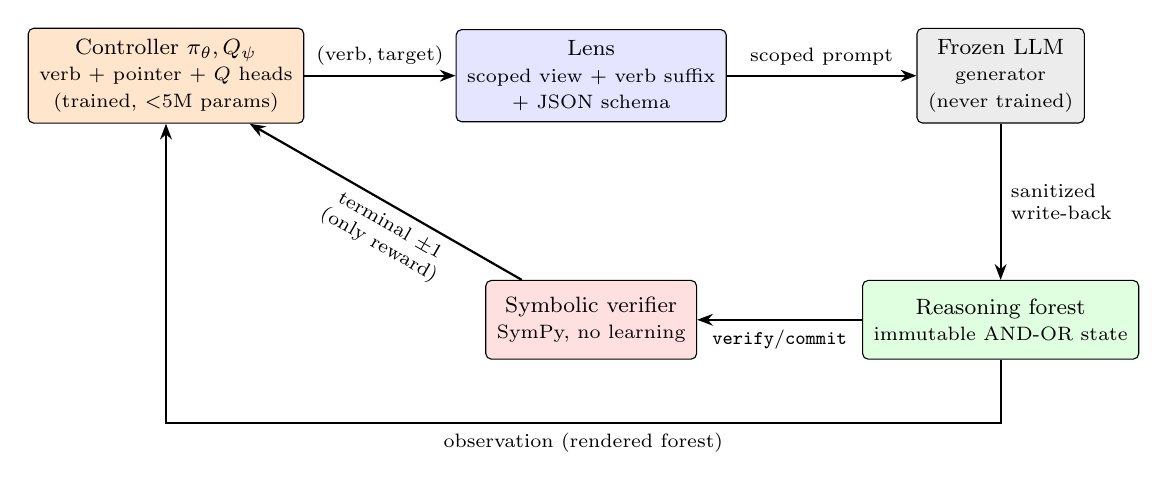
\begin{tikzpicture}[
      box/.style={draw, rounded corners=2pt, align=center, minimum height=10mm,
                  inner sep=4pt, font=\footnotesize},
      lab/.style={font=\scriptsize},
      arr/.style={-{Stealth[length=2mm]}, thick}]
    \node[box, fill=orange!20] (ctrl) at (0,0)
      {Controller $\pitheta,\Qpsi$\\ \scriptsize verb + pointer + $Q$ heads\\ \scriptsize (trained, $<$5M params)};
    \node[box, fill=blue!10] (lens) at (5.4,0)
      {Lens\\ \scriptsize scoped view + verb suffix\\ \scriptsize + JSON schema};
    \node[box, fill=gray!15] (llm) at (10.6,0)
      {Frozen LLM\\ \scriptsize generator\\ \scriptsize (never trained)};
    \node[box, fill=green!12] (forest) at (10.6,-3.1)
      {Reasoning forest\\ \scriptsize immutable AND-OR state};
    \node[box, fill=red!12] (ver) at (5.4,-3.1)
      {Symbolic verifier\\ \scriptsize SymPy, no learning};

    \draw[arr] (ctrl) -- node[lab, above, midway] {$(\text{verb},\text{target})$} (lens);
    \draw[arr] (lens) -- node[lab, above, midway] {scoped prompt} (llm);
    \draw[arr] (llm) -- node[lab, right, midway, align=left]
      {sanitized\\ write-back} (forest);
    \draw[arr] (forest) -- node[lab, below, midway]
      {\verbword{verify}/\verbword{commit}} (ver);
    \draw[arr] (ver) -- node[lab, sloped, below, pos=0.45, align=center]
      {terminal $\pm 1$\\ (only reward)} (ctrl);
    \draw[arr] (forest.south) -- ++(0,-0.8)
      -| node[lab, below, pos=0.25] {observation (rendered forest)} (ctrl.south);
  \end{tikzpicture}

  \medskip
  \footnotesize
  \verbword{verify}/\verbword{commit}/\verbword{abandon} make \alert{no LLM
  call}: the policy can neither author what is checked nor what it is checked
  against.
\end{frame}

% ---------------------------------------------------------------- state
\begin{frame}{State: a nested AND-OR reasoning forest}
  \centering
  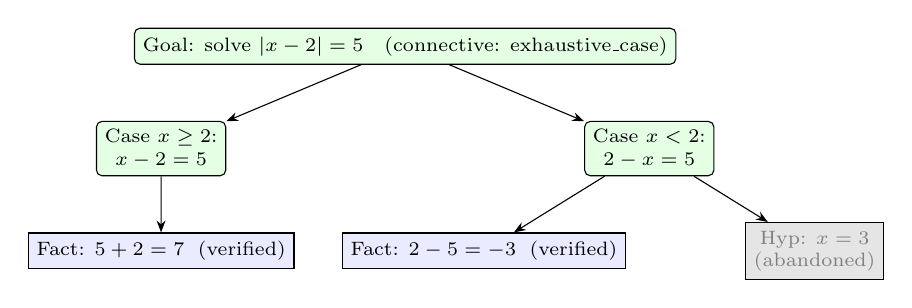
\begin{tikzpicture}[
      level distance=13mm,
      level 1/.style={sibling distance=62mm},
      level 2/.style={sibling distance=42mm},
      g/.style={draw, rounded corners=2pt, align=center, font=\scriptsize,
                inner sep=3pt, fill=green!10},
      f/.style={draw, align=center, font=\scriptsize, inner sep=3pt, fill=blue!8},
      dead/.style={draw, align=center, font=\scriptsize, inner sep=3pt,
                   fill=gray!20, text=gray},
      edge from parent/.style={draw, -{Stealth[length=1.5mm]}}]
    \node[g] {Goal: solve $|x-2| = 5$ \; \scriptsize(connective: exhaustive\_case)}
      child {node[g] {Case $x \ge 2$:\\ $x - 2 = 5$}
        child {node[f] {Fact: $5 + 2 = 7$ \;(verified)}}
      }
      child {node[g] {Case $x < 2$:\\ $2 - x = 5$}
        child {node[f] {Fact: $2 - 5 = -3$ \;(verified)}}
        child {node[dead] {Hyp: $x = 3$\\ (abandoned)}}
      };
  \end{tikzpicture}

  \medskip
  \begin{itemize}
    \item Frozen dataclasses: \texttt{Goal}, \texttt{Hypothesis},
          \texttt{Fact}, \texttt{VerifierCall}; verbs are total functions
          $\text{Graph} \to \text{Ok} \mid \text{Err}$
    \item No reward or value stored in nodes; \texttt{solved}/\texttt{verified}
          are derived predicates
    \item Structure never gates: the connective is metadata for the
          controller, not a hard rule
    \item Closed subtrees compact to one line in every rendered view
          (built-in roll-back / summarize)
  \end{itemize}
\end{frame}

% ---------------------------------------------------------------- actions
\begin{frame}{Action space: six verbs, one pointer}
  \begin{center}
    \footnotesize
    \begin{tabular}{lll}
      \toprule
      Verb & LLM call? & Effect \\
      \midrule
      \verbword{split} & yes & decompose a goal into subgoals or exhaustive cases \\
      \verbword{form\_hypothesis} & yes & add a tentative claim under a goal \\
      \verbword{compute} & yes & add one checkable ground equation as a fact \\
      \verbword{verify} & \alert{no} & run the symbolic checker on a node's statement \\
      \verbword{commit} & \alert{no} & close a goal on verifier-vouched evidence \\
      \verbword{abandon} & \alert{no} & prune a dead end (excluded from menus and views) \\
      \bottomrule
    \end{tabular}
  \end{center}
  \begin{block}{The lens property}
    Choosing $(\text{verb}, \text{target})$ simultaneously picks the
    operation \emph{and} the slice of state the frozen generator sees:
    problem + ancestor path + target subtree, siblings hidden, closed
    subtrees compacted. Write-back is local and sanitized against marker
    injection.
  \end{block}
\end{frame}

% ---------------------------------------------------------------- reward + training
\begin{frame}{Reward invariant and the training ladder}
  \begin{columns}[T]
    \begin{column}{0.48\textwidth}
      \textbf{Reward (load-bearing)}
      \begin{itemize}
        \item Terminal $+1/-1$ at root \verbword{commit}; $0$ elsewhere
        \item Masked/illegal action: small penalty
        \item No learned reward of any kind, ever
        \item Aesthetic signals may enter only as search priors, never as
              Bellman targets
      \end{itemize}
    \end{column}
    \begin{column}{0.48\textwidth}
      \textbf{Three rungs}
      \begin{enumerate}
        \item \alert{LLM-as-controller}: a strong teacher picks
              $(\text{verb},\text{target})$; JSONL trajectories logged
        \item Behavior cloning: warm-start $\pitheta$ on rung-1 data
        \item $Q$-learning fine-tune: off-policy, n-step / MC returns from
              the verifier; MCTS optional for better targets
      \end{enumerate}
    \end{column}
  \end{columns}
  \medskip
  \footnotesize
  Design-true collection regime: API teacher decides, a \emph{local small
  generator} writes all content, so trajectories reflect the deployed
  model's state distribution.
\end{frame}

% ---------------------------------------------------------------- prior art 1
\begin{frame}{Prior art: the landscape}
  \footnotesize
  \begin{center}
    \begin{tabular}{lll}
      \toprule
      Cluster & Exemplars & How we differ \\
      \midrule
      Search + train the LLM & TS-LLM, GSoS, OREO, & LLM frozen; controller \\
      \; (distill / fine-tune) & Agent Q, rStar-Math & is external and tiny \\
      \addlinespace
      Learned process reward & ReST-MCTS*, rStar-Math, & symbolic verifier is \\
      & V-STaR, TS-LLM (ORM) & the \emph{only} reward \\
      \addlinespace
      Prompt-level RL over & RLPrompt, TEMPERA & multi-step typed ops + \\
      \; frozen LM & & pointer over a forest \\
      \addlinespace
      External module + & PNLC (value only), & discrete action policy, \\
      \; frozen LLM & UniR (logit level) & operation-level $Q$ \\
      \addlinespace
      Context control (concurrent) & Active Context Curation & 7B pruning policy vs \\
      & (2026) & $<$5M lens-as-byproduct \\
      \bottomrule
    \end{tabular}
  \end{center}
\end{frame}

% ---------------------------------------------------------------- prior art 2
\begin{frame}{Prior art: the three real threats, and what survives}
  \textbf{Threats a reviewer will raise}
  \begin{enumerate}
    \item TS-LLM read as ``same loop, different reward source''
    \item ArCHer + GSoS + RLVR: ``each ingredient is published, the
          combination is engineering''
    \item Active Context Curation as concurrent work on the lens axis
  \end{enumerate}
  \medskip
  \textbf{What survives: the conjunction, claimed as such}
  \begin{itemize}
    \item Tiny \emph{external} controller (neither the LLM nor an LLM-sized critic)
    \item Factored verb + pointer heads over live node ids of a growing forest
    \item Off-policy value-based $Q$-learning as the spine, MCTS strictly additive
    \item Symbolic verifier as the sole reward, no learned value/PRM/ORM anywhere
    \item The lens property: action selection = context scoping, with local write-back
  \end{itemize}
  \smallskip
  \footnotesize Honest caveat: defensible but thin per-element; claim the
  conjunction, not a new RL algorithm.
\end{frame}

% ---------------------------------------------------------------- results 1
\begin{frame}{Rung 1 is live: teacher-as-controller on GSM8K}
  \begin{columns}[T]
    \begin{column}{0.52\textwidth}
      \textbf{Setup}
      \begin{itemize}
        \item gpt-4.1-mini as both controller-teacher and generator
        \item 247 GSM8K problems, depth limit 16, 3 workers,
              hard token budget
        \item Verifier: SymPy; ground equations only
      \end{itemize}
      \medskip
      \textbf{Headline numbers}
      \begin{itemize}
        \item \alert{71.7\%} solved (177/247)
        \item 1{,}942 decisions; 7 fallbacks (0.36\%)
        \item median 7 turns; pilot cost $<$ \$0.20
      \end{itemize}
    \end{column}
    \begin{column}{0.44\textwidth}
      \textbf{Verb usage (1{,}942 decisions)}
      \begin{center}
        \footnotesize
        \begin{tabular}{lr}
          \toprule
          \verbword{compute} & 1165 \\
          \verbword{verify} & 558 \\
          \verbword{commit} & 203 \\
          \verbword{split} & 7 \\
          \verbword{form\_hypothesis} & 5 \\
          \verbword{abandon} & 4 \\
          \bottomrule
        \end{tabular}
      \end{center}
      \medskip
      \footnotesize The verify-iterate loop works: failed checks are
      surfaced as \texttt{(verify failed xN)} and the teacher reformulates
      instead of retrying.
    \end{column}
  \end{columns}
\end{frame}

% ---------------------------------------------------------------- results 2
\begin{frame}{Diagnosis: healthy linear skill, collapsed structure}
  \begin{itemize}
    \item The dominant trajectory is \verbword{compute} $\to$
          \verbword{verify} $\to$ \verbword{commit}: correct play, because
          \alert{GSM8K is linearly solvable}
    \item Structural verbs (\verbword{split}, \verbword{abandon}) appear in
          under 1\% of decisions: behavior cloning on this data alone would
          learn a linear-chain policy
    \item This is a \emph{dataset} property, not a system failure: the AND-OR
          forest never earns its keep on problems with no cases
  \end{itemize}
  \begin{block}{The fix: generate our own problems}
    The verifier can \emph{decide} answers (SymPy solves the task), so we can
    generate problems in reverse: choose the case structure and answer set
    first, synthesize the statement around it. Ground truth by construction,
    unlimited scale, difficulty as a curriculum knob. Absolute values,
    piecewise casework, inequalities, ``find all solutions'': each makes
    \verbword{split} and \verbword{abandon} genuinely optimal.
  \end{block}
\end{frame}

% ---------------------------------------------------------------- next steps
\begin{frame}{Next steps}
  \begin{enumerate}
    \item \textbf{Finish the GSM8K sweep} (problems 247-499, running now)
    \item \textbf{Synthetic casework generator}: SymPy-verified structured
          problems + a structure-encouraging teacher prompt; contrast batch
          so \verbword{split}/\verbword{abandon} appear in BC data
    \item \textbf{Design-true regime}: API teacher + local small generator
          (Qwen 1.5B/3B); measure the small model's masked-action rate first
    \item \textbf{Phase B}: per-node encoder + pointer head, BC warm-start on
          rung-1 trajectories, then $Q$-learning fine-tune against the
          verifier
  \end{enumerate}
  \medskip
  \begin{block}{One-sentence summary}
    Search and scale live in the teacher and the compute knob; what we
    \emph{learn} is a tiny verifier-anchored controller over a frozen LLM.
  \end{block}
\end{frame}

\end{document}
